\documentclass[11pt]{article}
\usepackage[brazilian]{babel}
\usepackage[utf8x]{inputenc}
\usepackage[a4paper, total={6in, 8in}]{geometry}
\usepackage{enumitem}
\usepackage{pgfplots}
\usepackage{graphicx} 
\usepackage{float}
\pgfplotsset{width=10cm, compat=1.9}
\usepackage[framed,numbered,useliterate]{mcode}
\setlength{\parindent}{4em}
\renewcommand{\lstlistingname}{Código}

\begin{document}
\author{
	José Fernando Rosa Ribeiro
}
\title{DAS5210 - Introdução ao Controle de Processos
	\newline
	\newline
	\large Prova 1
	\date{\vspace{-5ex}}}
\maketitle
\setcounter{secnumdepth}{0}

\section{Questão 1}

Em nosso sistema, desejamos controlar a velocidade angular $\omega(t)$ do eixo de rotação de um motor através da manipulação
da tensão do circuito de acionamento $u(t)$. A descrição do sistema consta nas instruções da prova,
motivo pelo qual não será objeto desse relatório. A nossa variável de controle aqui é $\omega(t)$, e atuaremos
sobre a variável manipulada $u(t)$ a fim de obter os valores desejados de $\omega(t)$, nunca deixando de levar
em conta eventuais perturbações do sistemea, aqui representados por $q(t)$.

A fim de iniciar, precisamos montar o sistema não linearizado no ambiente de modelagem de sistemas dinâmicos Simulink.
A planta de malha aberta que obtive é a que se segue.
É importante ressaltar que esse modelo nada mais é do que uma representação no ambiente de modelagem das equações fornecidas.

Além disso, ressalto que, como uma perturbação, $q(t)$ contribui negativamente com o equilíbrio do sistema.
Por este motivo, a entrada do somador a que $q(t)$ está ligada é negativa.
Perturbações são sinais que podem interagir com o processo que estamos modelando a ponto de interferir controle
do sistema de controle em questão.
A fim de garantir a qualidade do controle exercido, pode ser necessário levá-las em conta no desenho do nosso sistema.

\begin{figure}[H]
	\centering
	{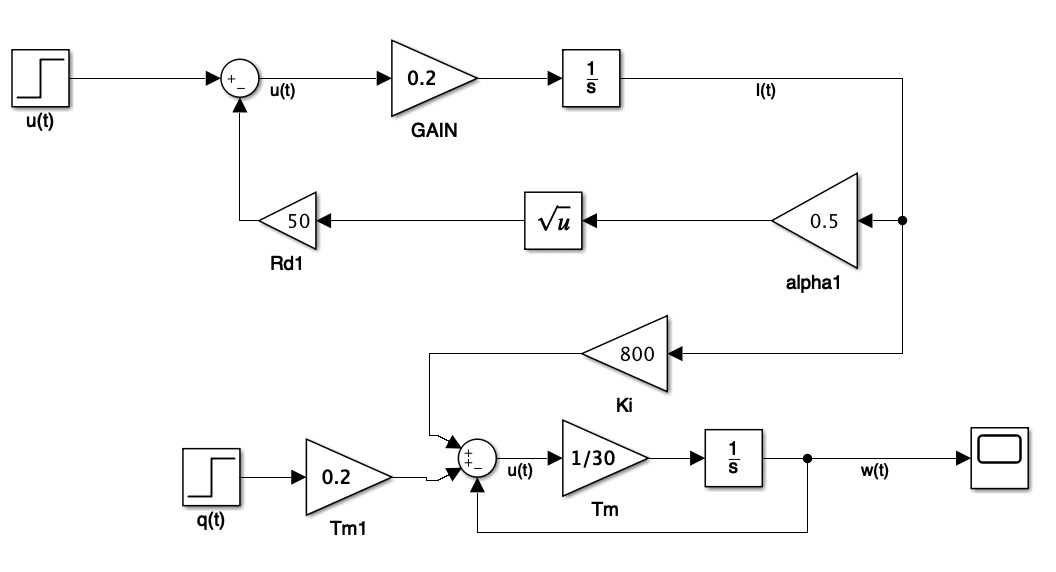
\includegraphics[width=\textwidth]
		{assets/q1_non_linearized_schema.jpg}}
	\caption{Diagrama do sistema não-linearizado no Simulink.}
\end{figure}

\begin{figure}[H]
	\centering
	{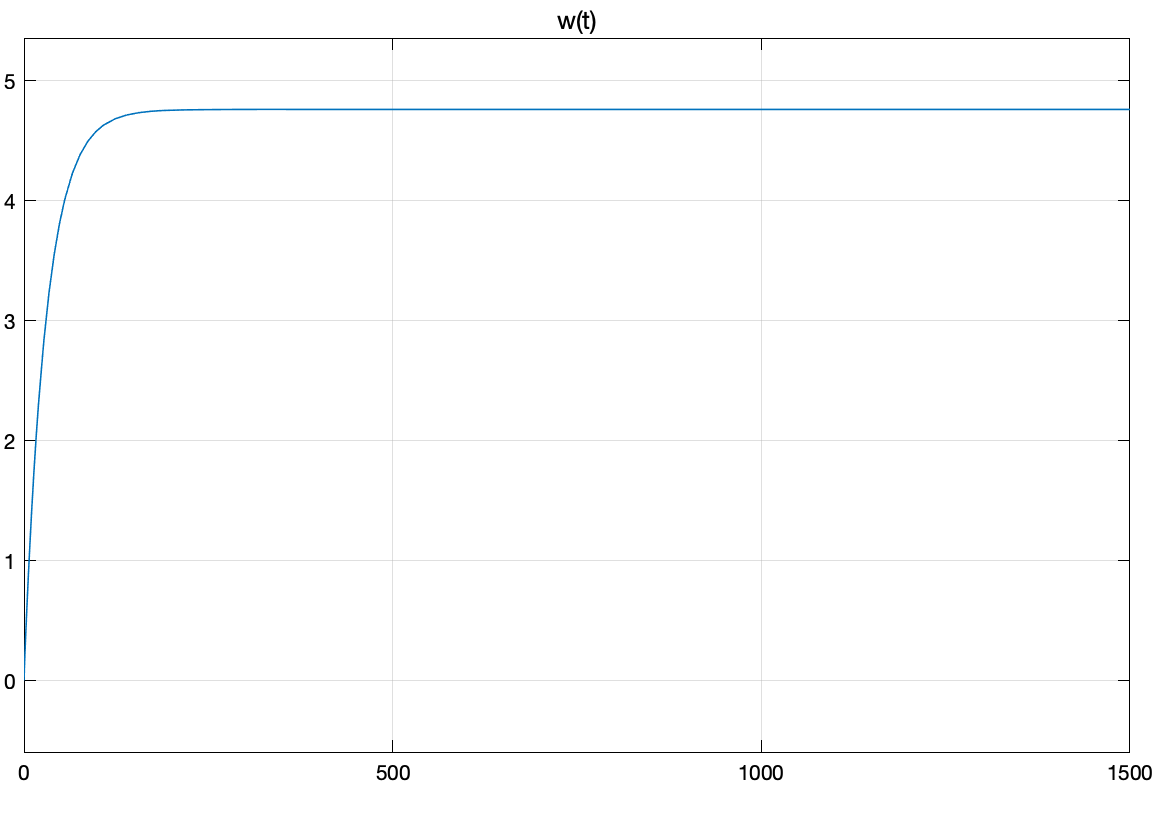
\includegraphics[width=0.5\textwidth]
		{assets/q1_u(t)_3_q(t)_0to5.png}}
	\caption{Gráfico da variação de $\omega(t)$ com u(t)=5 e degrau q(t-1)=5}
\end{figure}

\begin{figure}[H]
	\centering
	{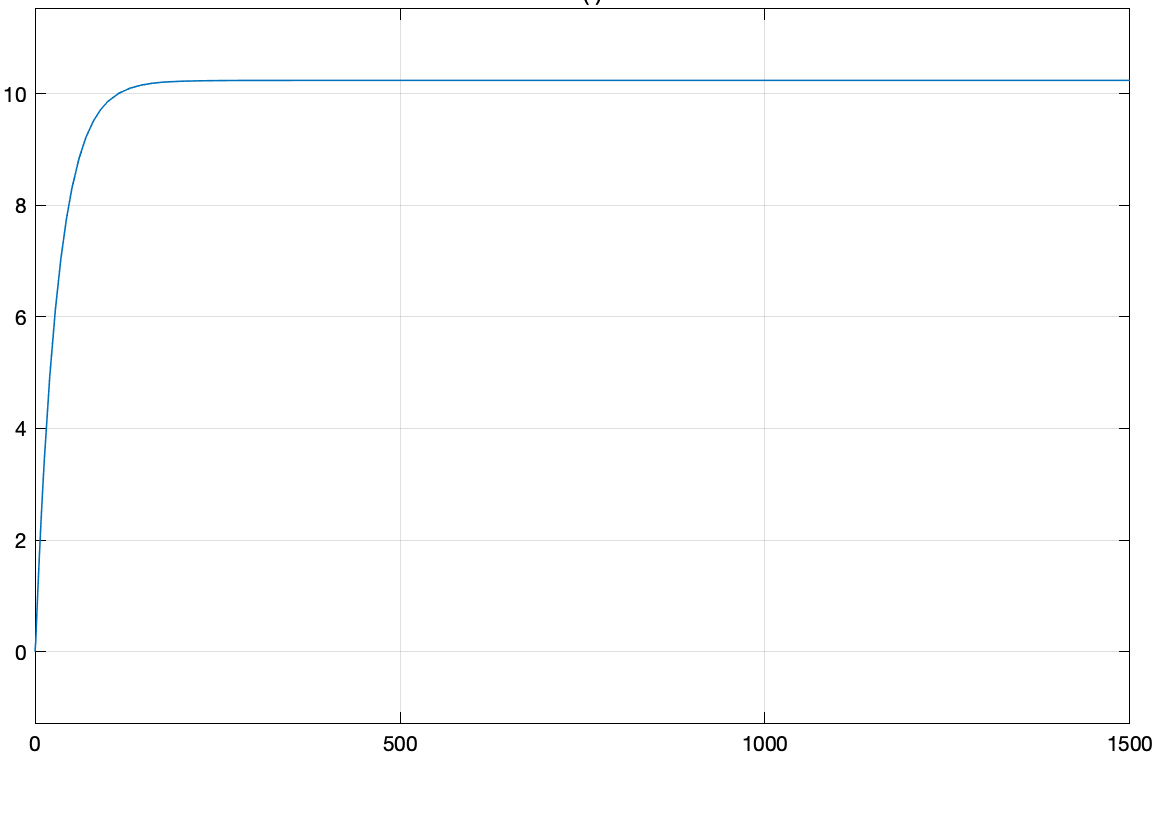
\includegraphics[width=0.5\textwidth]
		{assets/q1_u(t)_3to4_q(t)_0.png}}
	\caption{Gráfico da variação de $\omega(t)$ com degrau u(t-1)=3 a 4 e q(t)=0}
\end{figure}

\begin{figure}[H]
	\centering
	{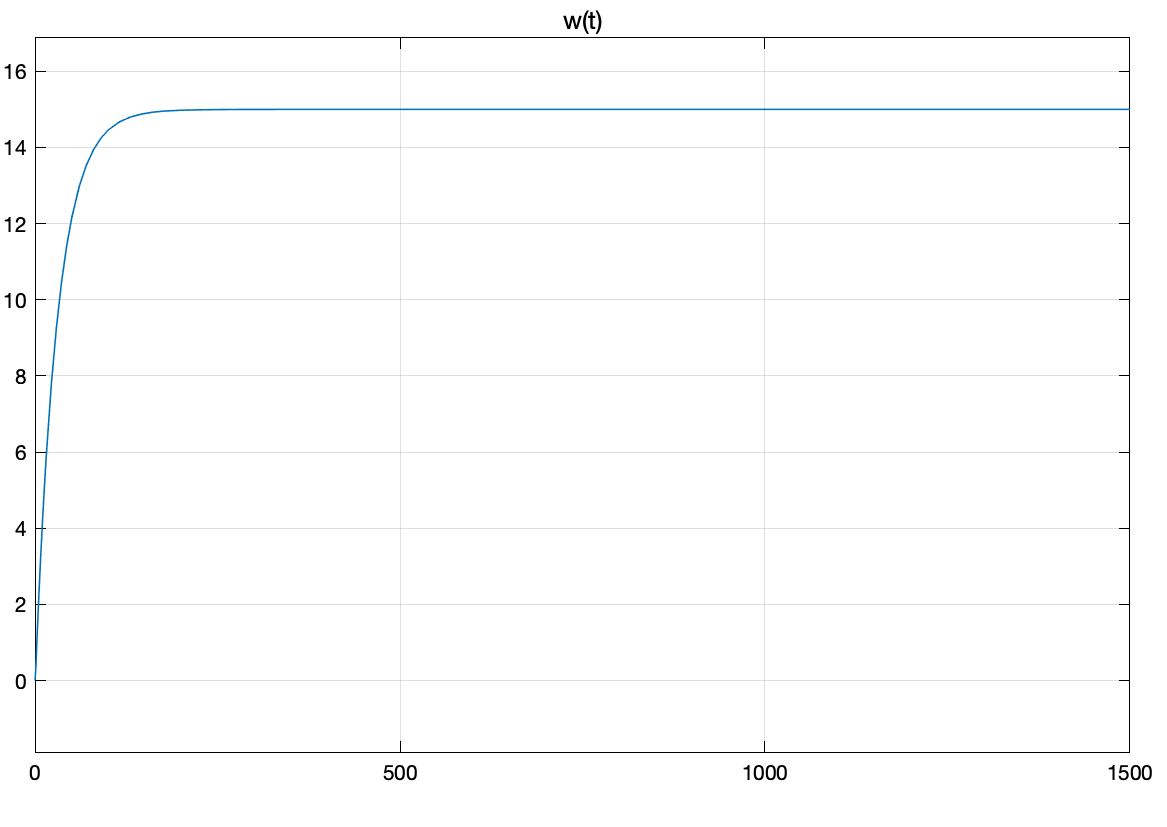
\includegraphics[width=0.5\textwidth]
		{assets/q1_u(t)_4to5_q(t)_5.png}}
	\caption{Gráfico da variação de $\omega(t)$ com u(t-1)=4 a 5 e q(t)=5}
\end{figure}

Podemos observar que os pontos de convergência para $\omega(t)$ variam bastante com o nível de perturbação
presente no sistema.

\section{Questão 2}
Dada a equação linearizada
\begin{equation}
	\zeta_{L}\frac{d\Delta i(t)}{dt} + \Delta i(t) = K_{L}\Delta u (t)
\end{equation}
montamos o sistema:
\begin{figure}[H]
	\centering
	{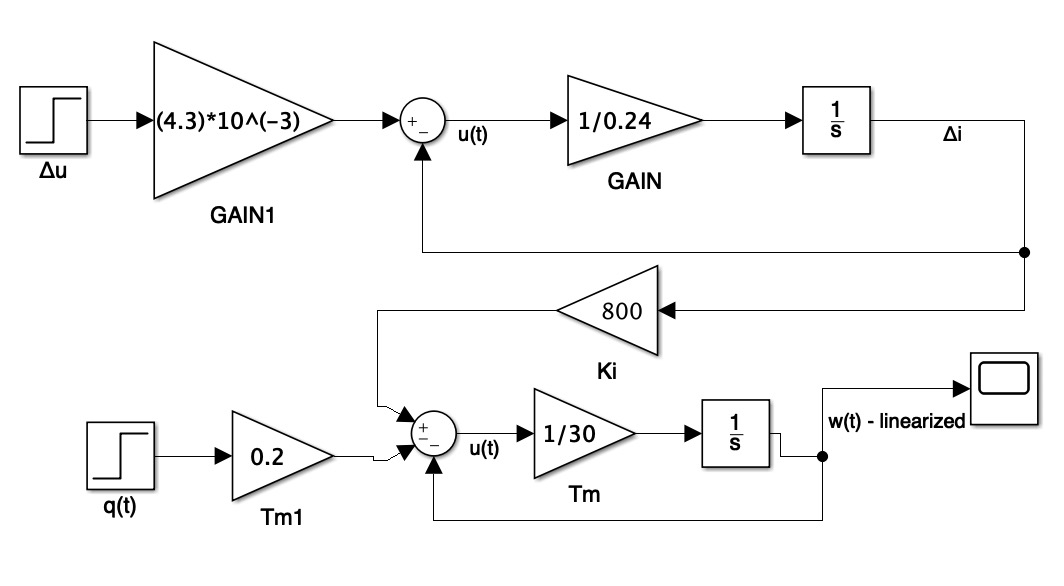
\includegraphics[width=\textwidth]
		{assets/q2_linearized_schema.jpg}}
	\caption{Diagrama do sistema linearizado.}
\end{figure}

\section{Questão 3}

Podemos observar através da figura que os valores do sistema linarizado não distam muito daqueles da forma
não-linearizada. No entanto, não se espera que essa linearização seja precisa para todo o domínio $i(t) \in [0, 20]mA$.
É esperado que ela seja tão precisa quanto mais perto estivermos do ponto de equilíbrio escolhido $i = 7.2mA$.

\begin{figure}[H]
	\centering
	{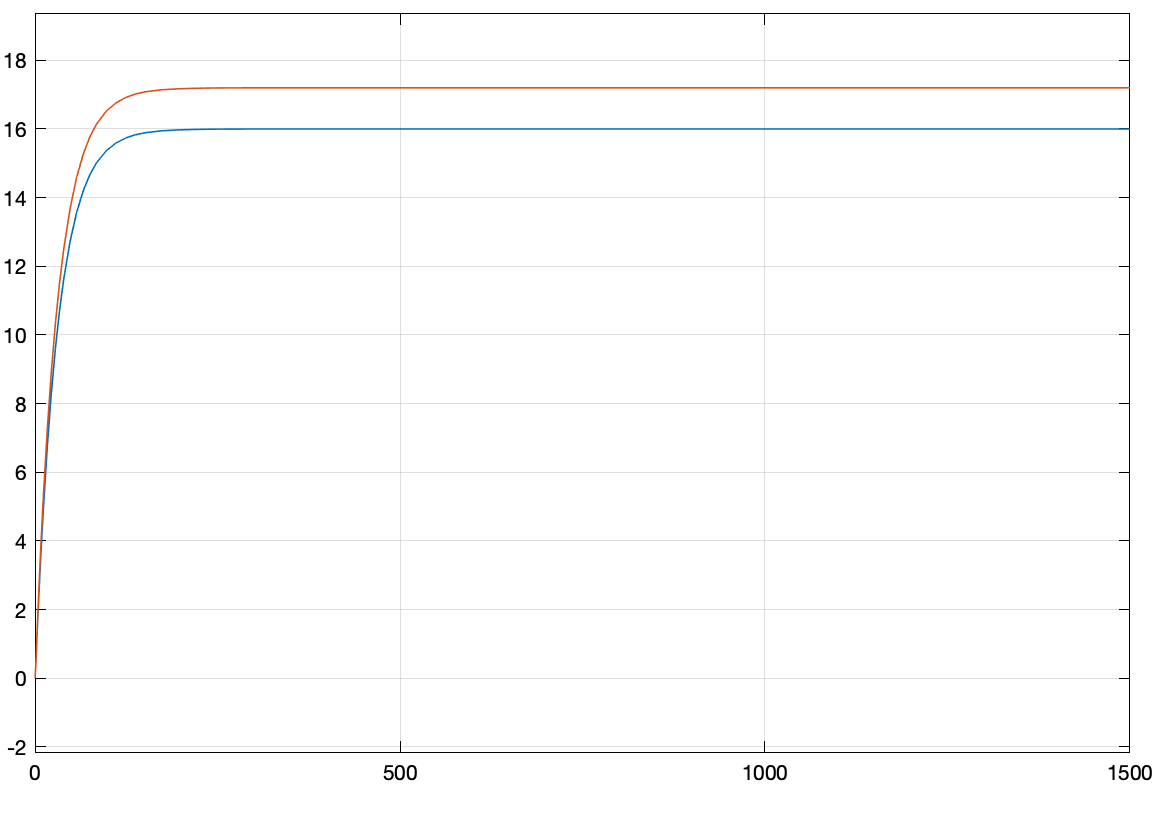
\includegraphics[width=\textwidth]
		{assets/q3_u(t)_4to5_q(t)_0to1+4.png}}
	\caption{Gráfico da comparação entre o sistema nas formas linearizada e não-linearizada.}
\end{figure}

\section{Questão 4}
\subsection{Itens a e b}
Tanto o código utilizado para estudar a simulação do sistema qunato a o esquema da planta no Simulink serão
úteis para os próximos da questão 4. O código a seguir está implantado na nossa planta no bloco $fcn$. Esse bloco
tem duas entradas e duas saídas. Como entrada, ele recebe tanto com o estado atual de $\omega(t)$
como uma informação da memória sobre a atuação sobre o bloco. A saída dessa função envia o sinal de atuação em $u(t)$
e salva na memória o estado da atuação (ativa ou não). Essa foi a solução encontrada para a implementação de uma
estratégia de controle on/off da velocidade angular que a mantivesse entre $5$ e $15$ $rad/s$.

O controle é ativado quando a velocidade se encontra abaixo de $5 rad/s$. Quando está ativo, envia $u(t) = 5V$
a fim de retomar $\omega(t) = 15 rad/s$. Neste patamar, desativamos o controle sobre a nossa variável manipulada
$u(t)$, até que a velocidade angular se encontre novamente abaixo de $5 rad/s$.
Cabe ressaltar que este sistema envia $u(t) = 1V$ quando o controle está inativo a fim de que não encontremos valores
negativos no nosso sistema, o que violaria o domínio da função $V_D(t)$.

\begin{lstlisting}[caption={Código usado para controlar a planta},captionpos=b]
function [y1, y2]= fcn(u, m)

	lower_bound = 5;
	upper_bound = 15;
	active = m;

	if active
			y1 = 5;
	else
			y1 = 1;
	end

	if u>=upper_bound
			active = 0;
	elseif u<=lower_bound
			active = 1;
	end

	y2 = active;
\end{lstlisting}

\begin{figure}[H]
	\centering
	{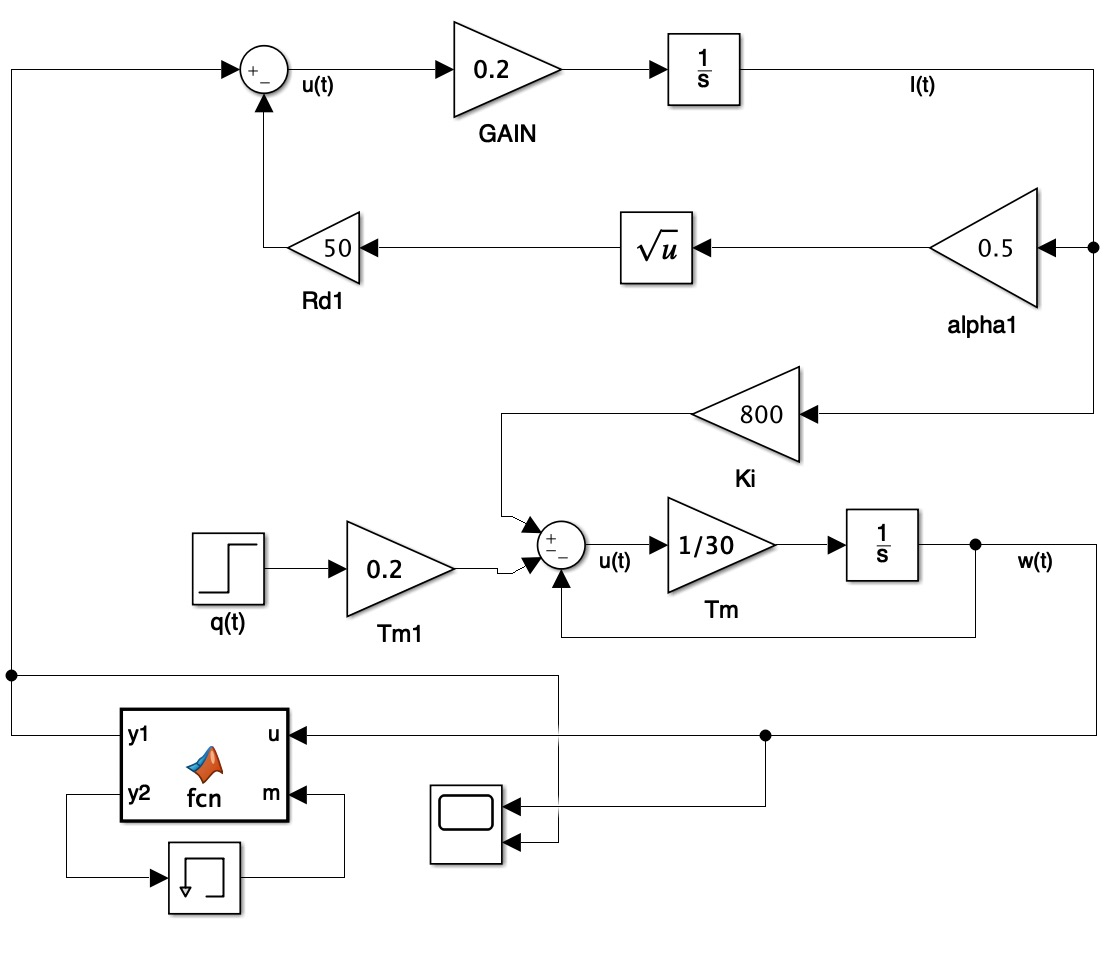
\includegraphics[width=\textwidth]
		{assets/q4_ab_control_schema.jpg}}
	\caption{Esquema da planta no Simulink.}
\end{figure}

\subsection{Item a}

Podemos observar que neste gráfico as variáveis manipulada ($u(t)$) e controlada ($\omega(t)$) da planta para
$ \tau_{q} =90s $ e uma perturbação de $Q(t) = 1 N.m$.

\begin{figure}[H]
	\centering
	{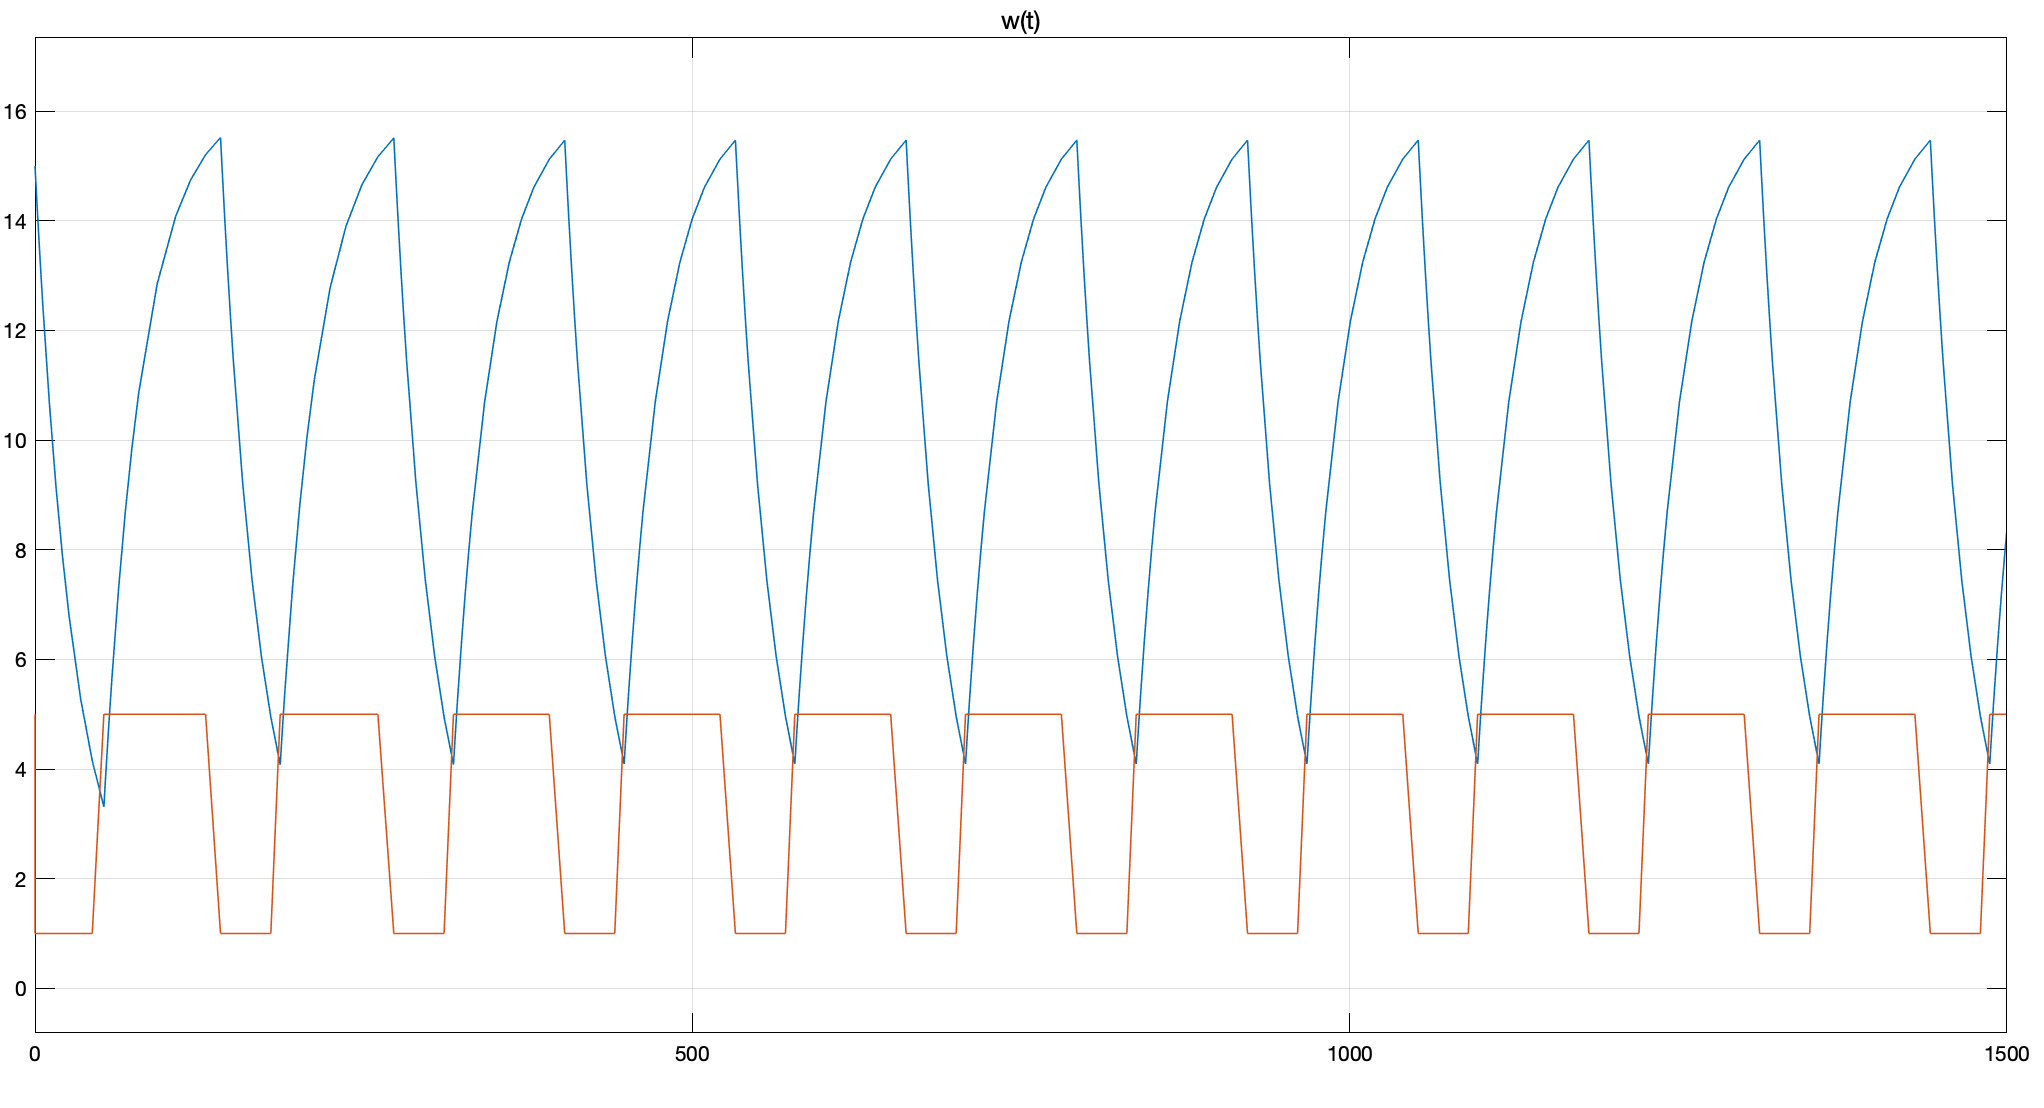
\includegraphics[width=\textwidth]
		{assets/q4_a_plot.png}}
	\caption{Gráfico de $u(t)$ (em vermelho) e $\omega(t)$ (em azul), respectivamente, para $Q(t) = 1 N.m$}
\end{figure}

\subsection{Item b}

Neste gráfico, fazemos uma simulação do sistema com os mesmos parâmetros que o anterior, alterando apenas
a perturbação $Q(t)$ para $Q(t) = 5 N.m$. É interessante notar como o tempo de atuação sobre a variável manipulada
aumenta sensivemente entre a situação anterior e a atual. Isso é esperado, pois aqui situação há uma maior
perturbação no sistema.

\begin{figure}[H]
	\centering
	{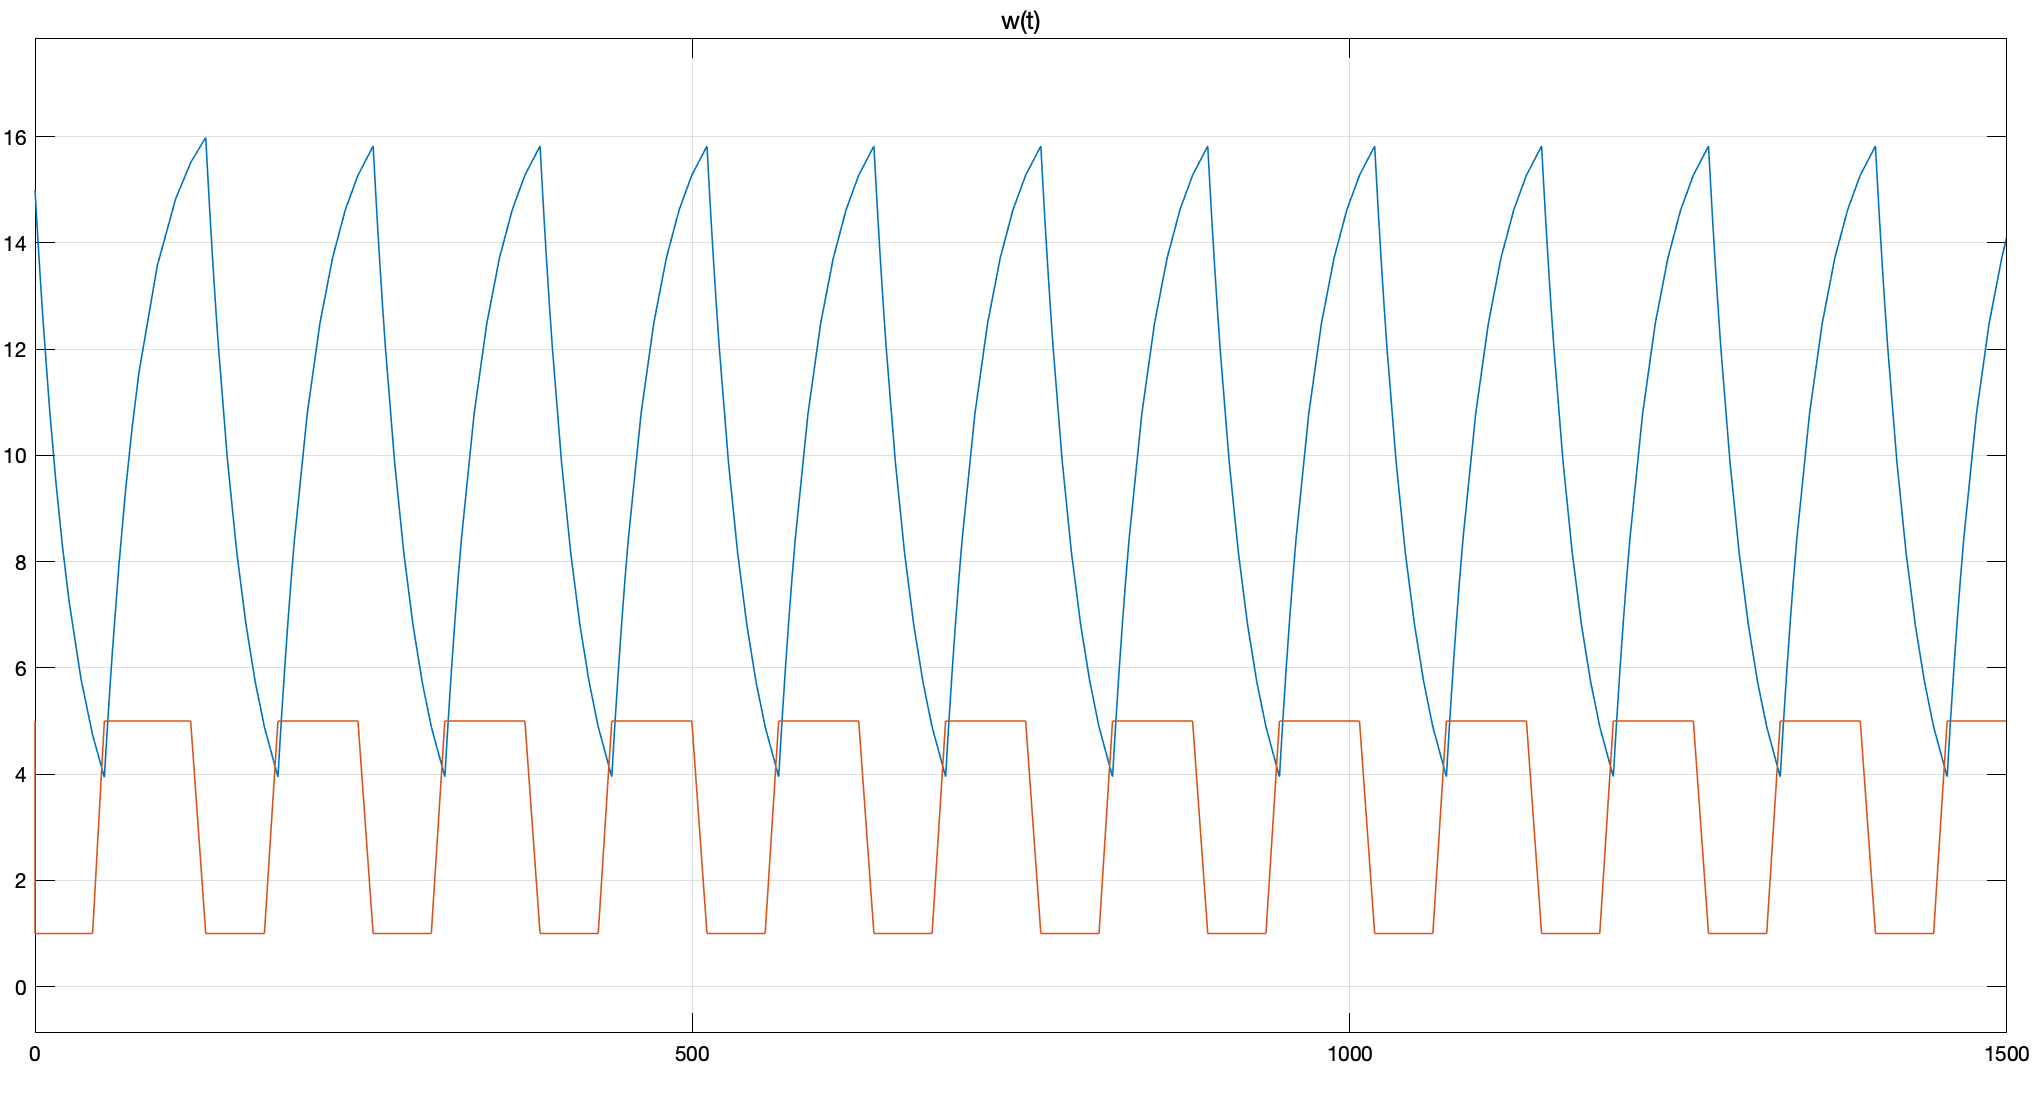
\includegraphics[width=\textwidth]
		{assets/q4_b_plot.png}}
	\caption{Gráfico de u(t) (em vermelho) e $\omega(t)$ (em azul), respectivamente, para $Q(t) = 5 N.m$}
\end{figure}

\subsection{Item c}

\begin{figure}[H]
	\centering
	{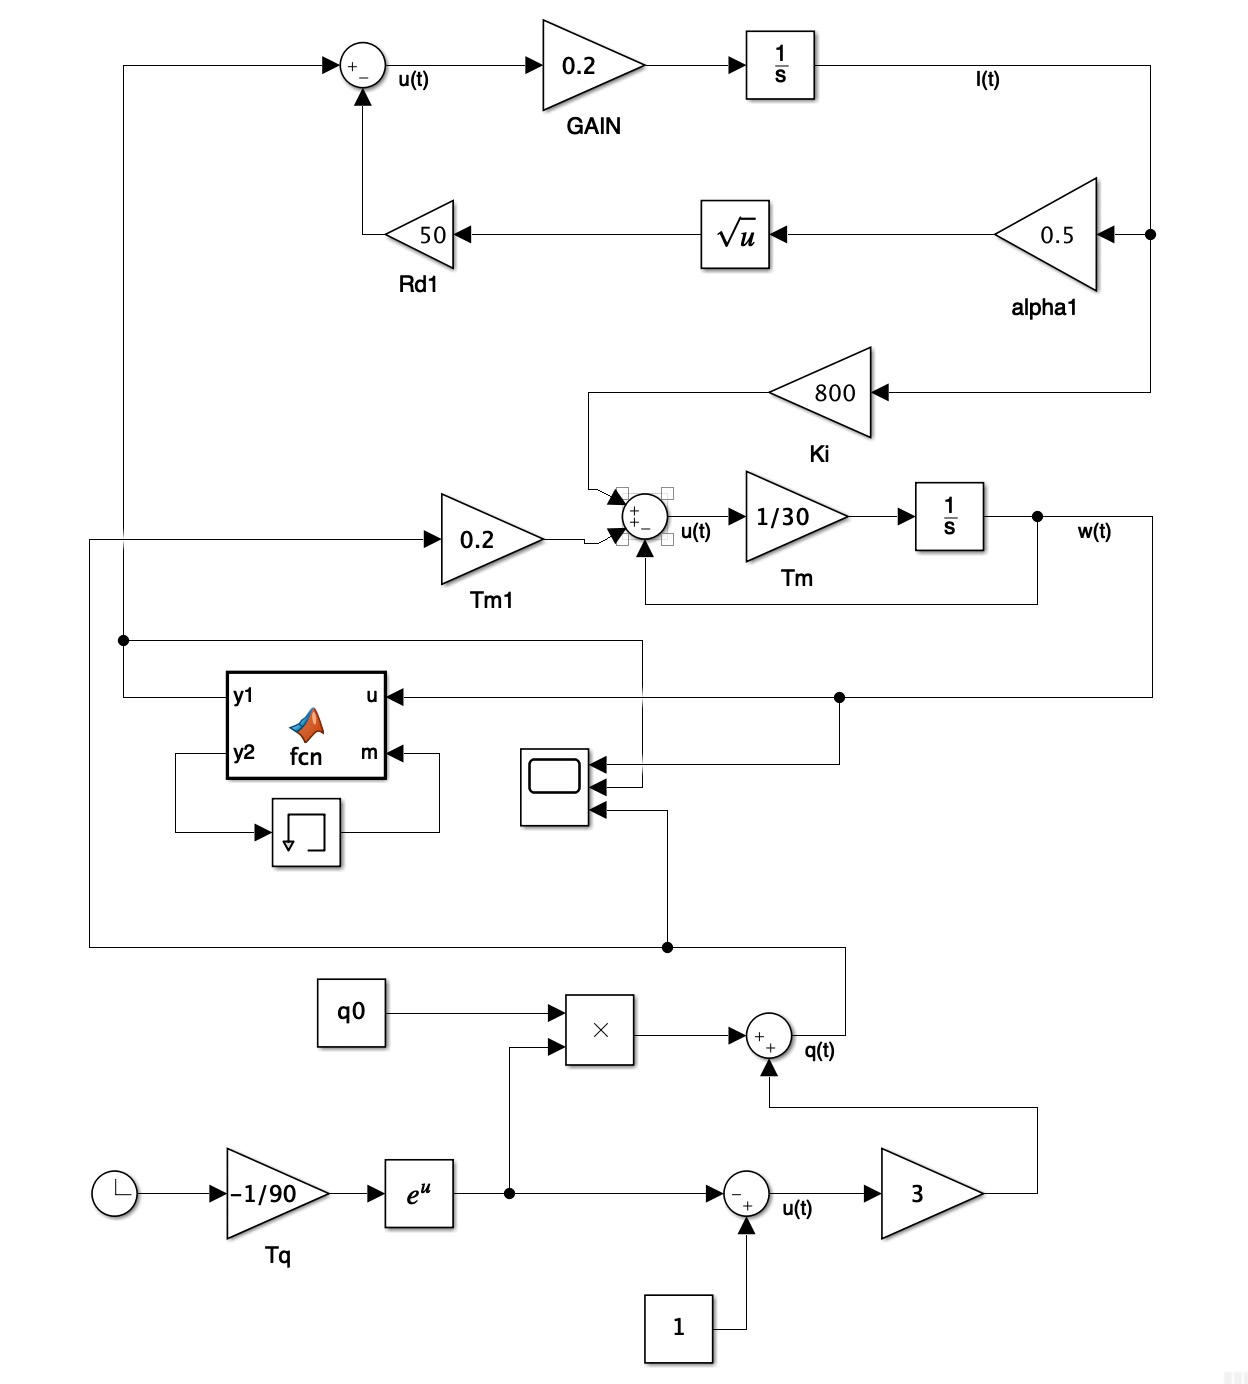
\includegraphics[width=\textwidth]
		{assets/q4_c_control_schema.jpg}}
	\caption{Esquema da planta no Simulink.}
\end{figure}

\begin{figure}[H]
	\centering
	{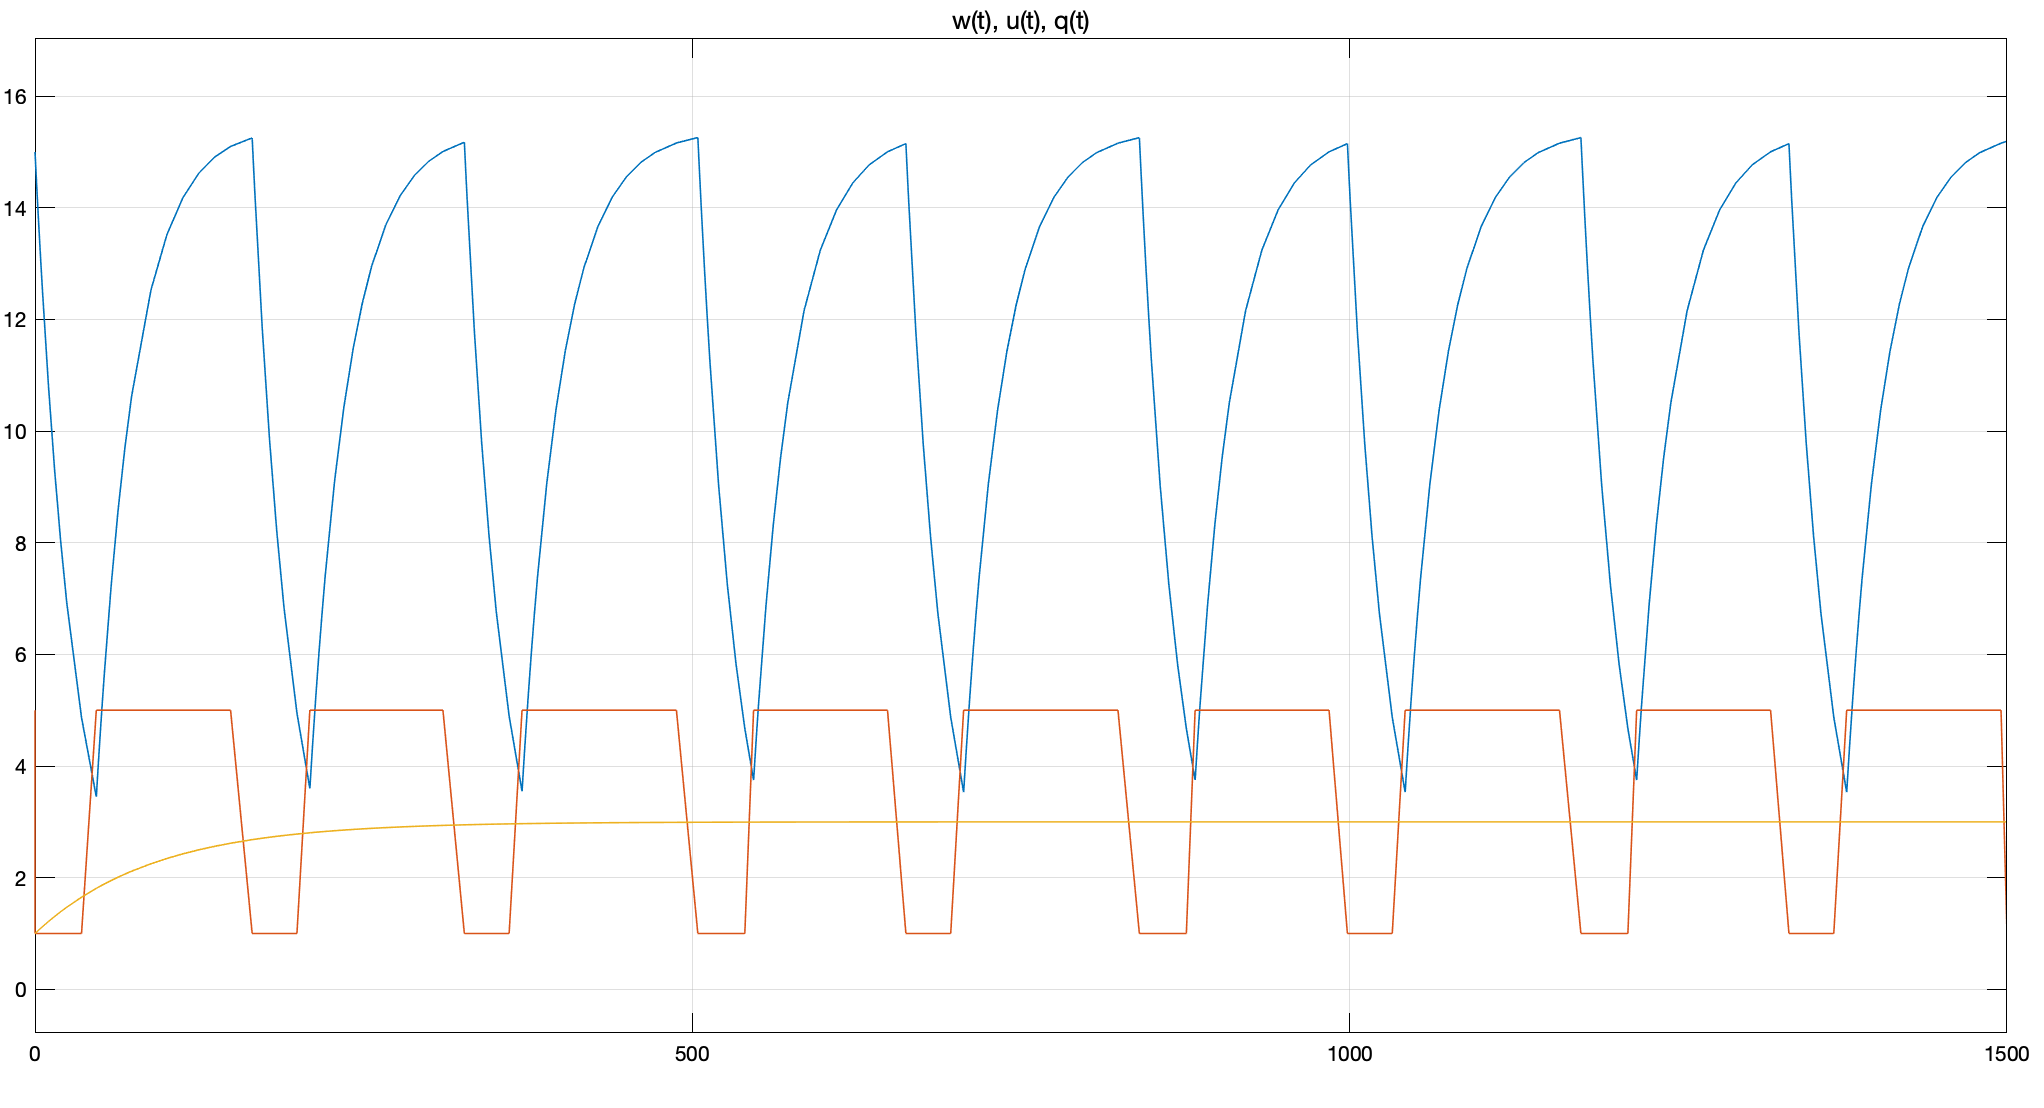
\includegraphics[width=\textwidth]
		{assets/q4_c_plot.png}}
	\caption{Gráfico de $u(t)$ (em vermelho) e $\omega(t)$ (em azul) e $q(t)$ (em amarelo.)}
\end{figure}


\section{Questão 5}

Sabemos que $V_{D}(t) + V_{L}(t) - u(t) = 0$. Mas como estamos em um ponto de equilíbrio,
$V_{L}(t) = L\frac{di}{dt}(t) = 0$. Portanto, $V_{D}(t) = u(t)$.

E sabemos que $i(t)$ está dado na relação $V_{D}(t) = R_{D}\sqrt{\alpha i(t)}$. Isolando $i(t)$, temos:

\begin{equation}
	(\frac{V_{D}(t)}{R_{D}})^2 . \frac{1}{\alpha} =  i(t)
\end{equation}

Como $V_{D}(t) = u(t)$, teremos $(\frac{u(t)}{R_{D}})^2 . \frac{1}{\alpha} =  i(t)$. Mas nos interessa controlar
a velocidade em malha aberta segundo a lei $u(t) = K_{MA}r(t)$. Teremos, portanto,

\begin{equation}
	(\frac{K_{MA}r(t)}{R_{D}})^2 . \frac{1}{\alpha} =  i(t)
\end{equation}

Como $\omega(t) = K_{i}i(t) + K_{q}q(t)$, pois estamos em um ponto de equilíbrio (isto é, $\frac{d\omega}{dt} = 0$),
teremos

\begin{equation}
	\omega(t) = K_{i}((\frac{K_{MA}r(t)}{R_{D}})^2 . \frac{1}{\alpha}) +  K_{q}q(t)
\end{equation}

Isolando $K_{MA}$:

\begin{equation}
	K_{MA} = \frac{R_{D}}{r(t)}\sqrt{\frac{\alpha(\omega(t) -  K_{q}q(t))}{K_{i}}}
\end{equation}

\begin{figure}[H]
	\centering
	{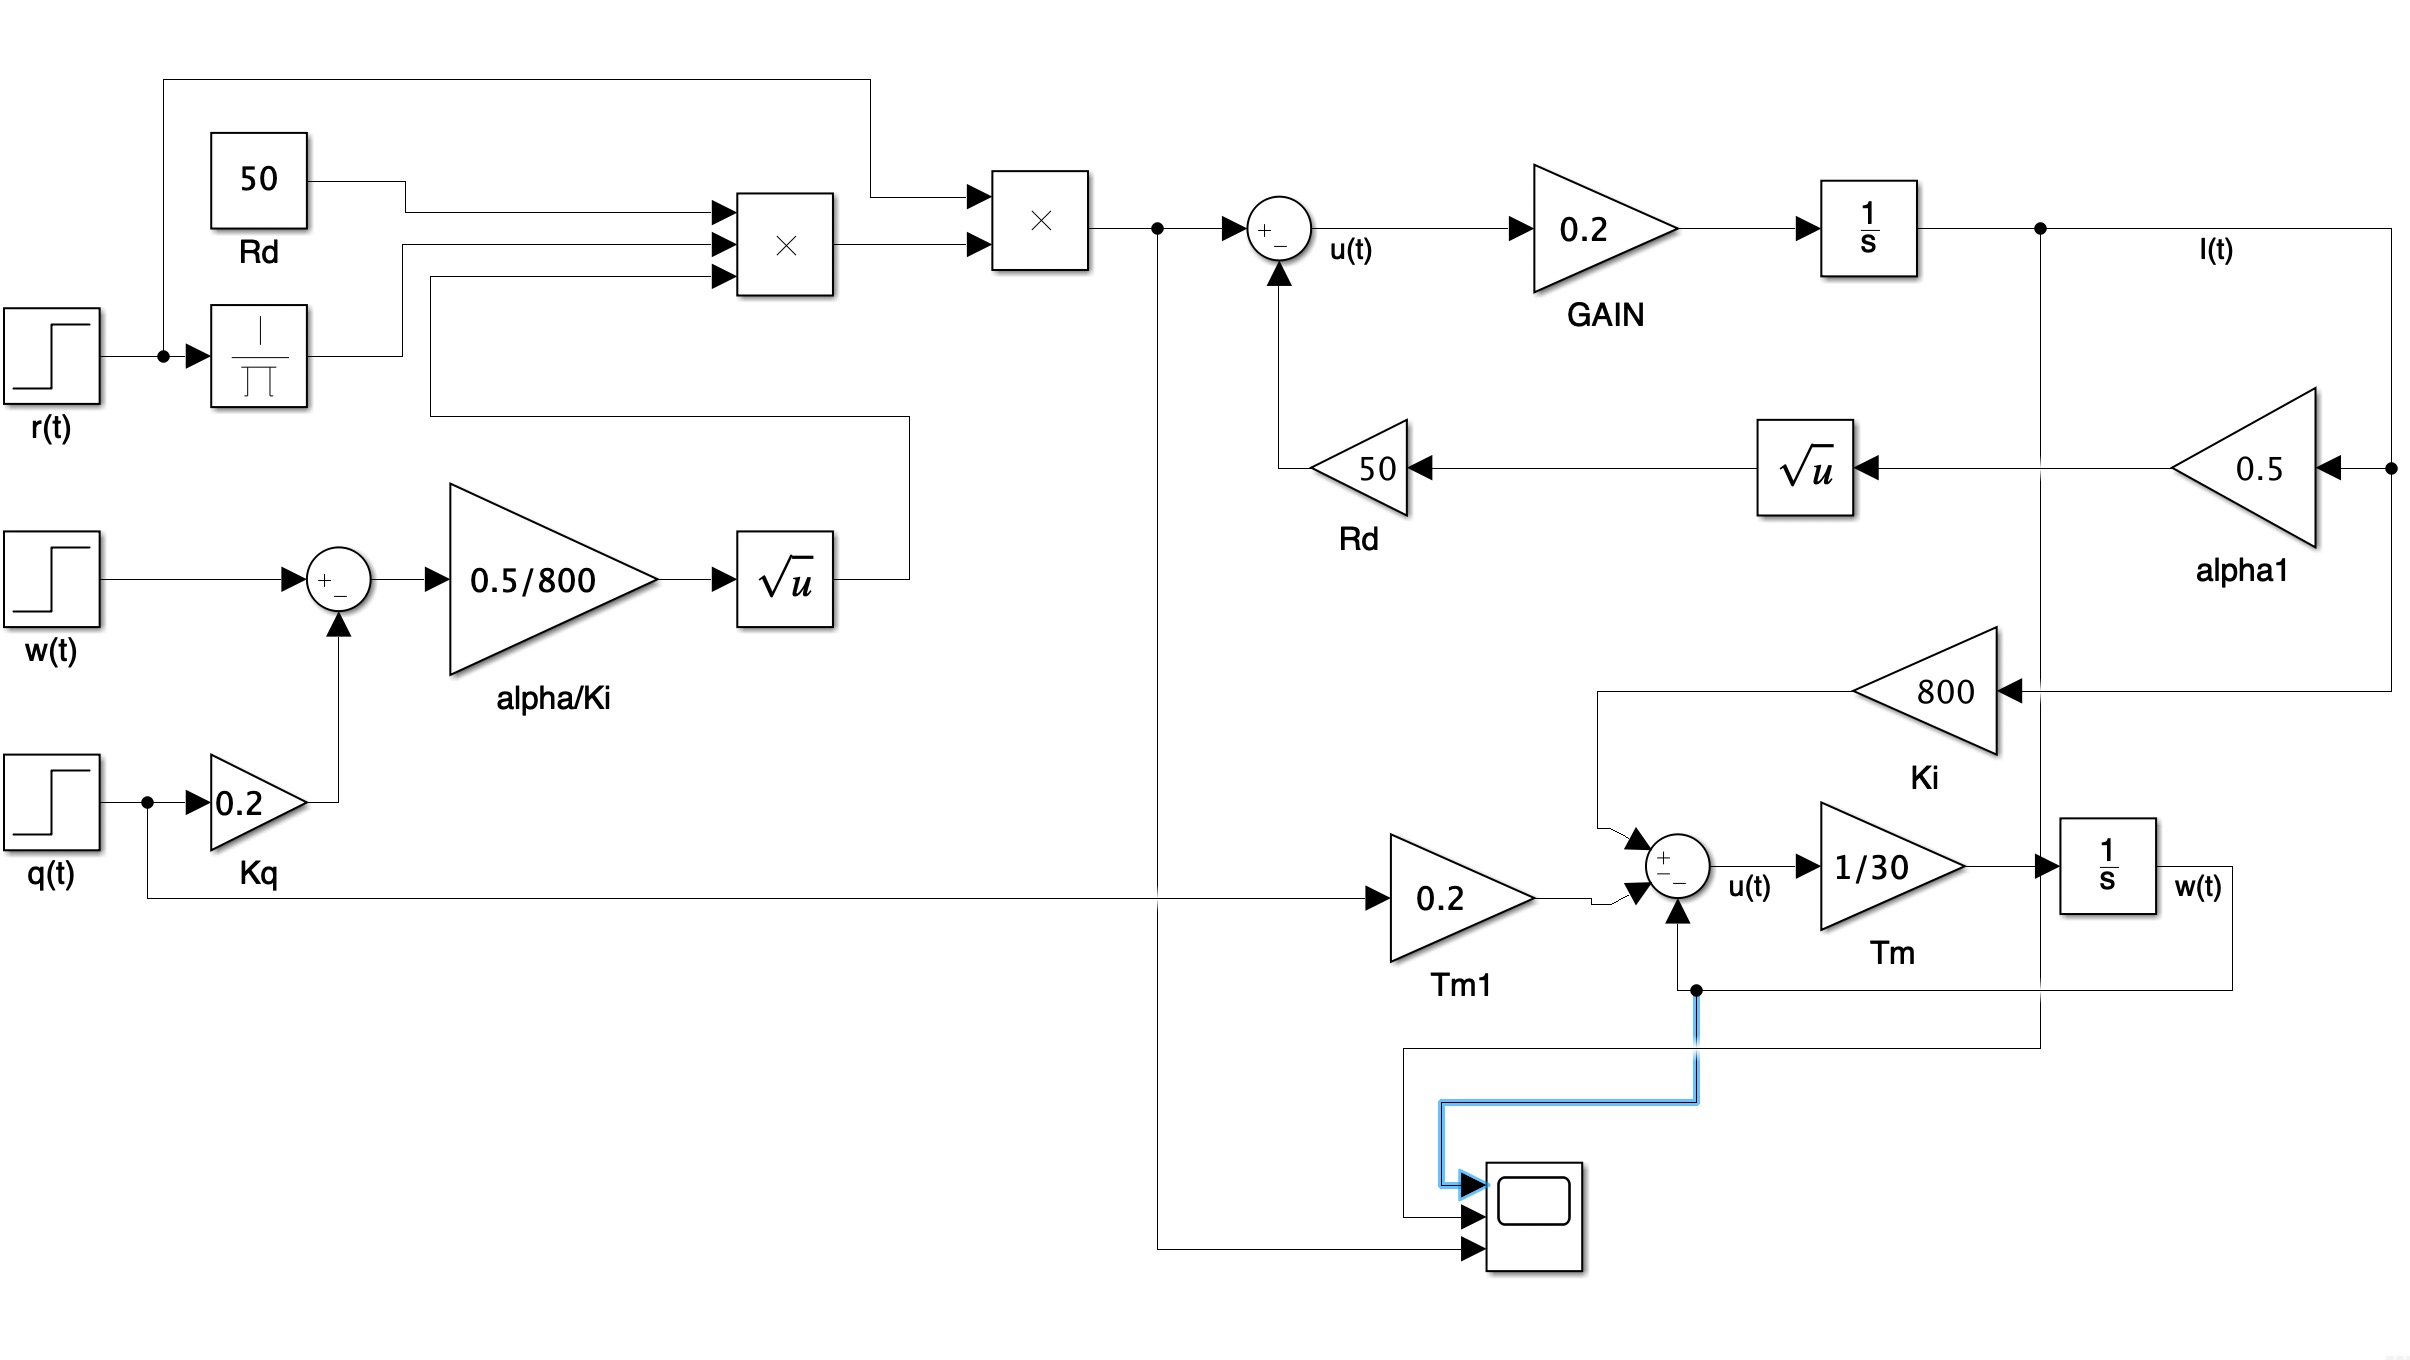
\includegraphics[width=\textwidth]
		{assets/q5.jpg}}
	\caption{Esquema da planta com controle de malha aberta no Simulink.}
\end{figure}

\section{Questão 6}
Em teoria, o controle em malha aberta torna o processo menos robusto em termos de rejeição de perturbações,
embora possa haver um maior seguimento de referência para sistemas sem perturbações.
A estratégia on-off, por ser realimentada, empresta mais robustez ao sistema a perturbações $q(t)$ do tipo degrau.
\end{document}
